\chapter{Barrier options}
\label{cap:barriere}

A barrier option is the first ``path-dependent'' exotic one meets: the final payment is that of a vanilla, but it
counts only if the underlying has (or has not) touched a given level during the life of the contract. In this chapter
we derive the closed-form formulas with the reflection principle, build a Monte Carlo free of monitoring error,
explain the Broadie--Glasserman--Kou correction for barriers observed on discrete dates, and see what changes under
Heston. At the end we report the numbers measured in the project.

\section{What they are}
A barrier option is a European call or put that is \textbf{activated} (\emph{knock-in}) or \textbf{extinguished}
(\emph{knock-out}) if the underlying touches a level $H$ before expiry. There are eight combinations
(Table~\ref{tab:barriere-tipi}).
\begin{table}[htbp]
\centering
\small
\caption{The eight barrier options.}
\label{tab:barriere-tipi}
\begin{tabularx}{\textwidth}{>{\raggedright\arraybackslash}Xll}
\toprule
barrier & knock-out (``out'') & knock-in (``in'')\\
\midrule
\emph{down} ($S_0>H$, touched from above) & down-and-out call/put & down-and-in call/put\\
\emph{up} ($S_0<H$, touched from below) & up-and-out call/put & up-and-in call/put\\
\bottomrule
\end{tabularx}
\end{table}

We abbreviate with three letters: c/p (call/put), d/u (down/up), i/o (in/out). For example, cdo is the down-and-out
call.

Notation. $\theta=+1$ for the call and $-1$ for the put; $\eta=+1$ for a down barrier and $-1$ for an up barrier. Let
$\tau=\inf\{t\ge0:\eta(S_t-H)\le0\}$ be the first hitting time. Then
\begin{equation}
\text{knock-out: }(\theta(S_T-K))^+\,\ind\{\tau>T\},\qquad
\text{knock-in: }(\theta(S_T-K))^+\,\ind\{\tau\le T\}.
\end{equation}
Sometimes there is a \emph{rebate} $R$, a fixed refund: the out option pays it at the hit, the in option pays it at
expiry if the barrier was never touched. In the main tests $R=0$.

\begin{idea}[title={Key idea: in + out = vanilla}]
On every path the barrier either was touched or was not: exactly one of knock-in and knock-out pays. Hence
\begin{equation}\label{eq:in-out}
\text{knock-in}+\text{knock-out}=\text{vanilla}\qquad(R=0),
\end{equation}
in \emph{any} model. In a Monte Carlo, if in and out are computed on the same paths and with the same weights, the
identity must hold \emph{to rounding}, not within statistical error. If it fails by one standard error, in and out are
using different paths or weights. Beware of the test as well: computing ``in $:=$ vanilla $-$ out'' would turn the
check into a tautology. The two legs must be priced with separate calls.
\end{idea}

\paragraph{Barrier on spot or on forward.} Contracts (and published tables) define $H$ on the index level $S_t$, not
on the forward. Our kernels, however, work on the forward $F_t=F(t,T)$. The link is a \textbf{constant carry} $b$
(the ``cost of carry'' $b=r-q$), which is a kernel input with default 0:
\begin{equation}\label{eq:spot-da-forward}
S_t=F_t\,e^{-b(T-t)},\qquad S_0=F\,e^{-bT},\qquad S_T=F_T .
\end{equation}
With $b=0$ the barrier sits directly on the forward. The rate $r=-\ln\DF/T$ is derived from $\DF$ and is needed only
for the rebate paid at the hit. One could put a constant barrier on $F_t$, but for $b>0$ this is equivalent to a
barrier on the spot that rises over time, and the published tables are not reproduced.

\section{The reflection principle}
It is the key tool for the closed-form formulas.
\begin{proposizione}[Reflection, driftless Brownian motion]
Let $W$ be a Brownian motion started at 0 and $\ell<0$ a level. For every $y\ge\ell$:
\begin{equation}
\PP\Big(\min_{[0,T]}W\le\ell,\ W_T\ge y\Big)=\PP\big(W_T\le2\ell-y\big).
\end{equation}
\end{proposizione}
\emph{Idea.} Take every path that touches $\ell$ and \emph{reflect} it about $\ell$ after the first hit. Brownian
motion restarts from $\ell$ without memory and is symmetric, so the reflected path is equally likely. A path that has
touched $\ell$ and ends above $y$ corresponds to one that ends below $2\ell-y$. Conversely, every path that ends below
$2\ell-y\le\ell$ must have touched $\ell$. The correspondence is one-to-one.

\subsection{With drift: three steps}
Under Black with carry $b$, from \eqref{eq:spot-da-forward} the spot log-price $Y_t=\ln(S_t/S_0)$ is a Brownian
motion with drift:
\[
Y_t=\nu t+\sigma W_t,\qquad \nu=b-\tfrac12\sigma^2 .
\]
The barrier becomes the constant level $\ell=\ln(H/S_0)$. We define
\begin{equation}
\varrho=\frac H{S_0}=\frac HF\,e^{bT},\qquad \mu=\frac b{\sigma^2}-\frac12=\frac\nu{\sigma^2},\qquad F^*=\varrho^2F .
\end{equation}
For a down barrier ($\ell<0$) and any function $f$ we want the expectation
\[
\E\big[f(Y_T);\ \min_{[0,T]} Y\le\ell,\ Y_T>\ell\big].
\]

\noindent\textbf{Step 1 (remove the drift).} By Girsanov there is a measure $\tilde\Q$ under which $Y$ is a
driftless Brownian motion, with
\[
\frac{\dd\Q}{\dd\tilde\Q}=\exp\Big(\frac{\nu}{\sigma^2}Y_T-\frac{\nu^2T}{2\sigma^2}\Big).
\]
The expectation we want is therefore
\[
\tilde\E\Big[e^{\mu Y_T-\nu^2T/(2\sigma^2)}f(Y_T);\ \text{hit},\ Y_T>\ell\Big].
\]

\noindent\textbf{Step 2 (reflect).} Under $\tilde\Q$ reflection holds: the event $\{\text{hit},\,Y_T>\ell\}$ maps onto
$\{Y_T<\ell\}$ and $Y_T$ becomes $2\ell-Y_T$. The weight $e^{\mu Y_T}$ becomes
$e^{\mu(2\ell-Y_T)}=e^{2\mu\ell}e^{-\mu Y_T}$.

\noindent\textbf{Step 3 (go back).} Under $\tilde\Q$, $Y\mapsto-Y$ is also a symmetry. Applying it, the weight
$e^{-\mu Y_T}$ turns back into $e^{+\mu Y_T}$, that is, the density of $\Q$ again, and the event becomes
$\{2\ell+Y_T>\ell\}$. Result:
\begin{equation}\label{eq:immagine}
\E\big[f(Y_T);\ \text{hit }\ell,\ Y_T>\ell\big]=\varrho^{2\mu}\,\E\big[f(2\ell+Y_T);\ 2\ell+Y_T>\ell\big],
\end{equation}
because $e^{2\mu\ell}=e^{2\mu\ln\varrho}=\varrho^{2\mu}$.

\begin{idea}[title={The reflected world}]
The right-hand side contains $S_0e^{2\ell+Y_T}=\varrho^2S_T$, whose expectation is $\varrho^2F=F^*$. The ``reflected
world'' is therefore a Black world with \textbf{image forward} $F^*$, weighted by $\varrho^{2\mu}$. Every barrier
price is a combination of Black formulas in the true world and in the reflected world.
\end{idea}

\section{The Reiner--Rubinstein closed-form formulas in forward form}
We introduce the ``truncated'' Black formula with forward $X$ and cut-off level $L$:
\[
G(X,L;\kappa)=\theta\,\DF\big[X\,\Phi(\kappa\,d_1(X,L))-K\,\Phi(\kappa\,d_2(X,L))\big],\qquad
d_{1,2}(X,L)=\frac{\ln(X/L)}{\sigma\sqrt T}\pm\frac{\sigma\sqrt T}2 .
\]
The four building blocks are
\begin{align*}
A&=G(F,K;\theta)=\text{vanilla}, & B&=G(F,H;\theta),\\
C&=\varrho^{2\mu}\,G(F^*,K;\eta), & D&=\varrho^{2\mu}\,G(F^*,H;\eta).
\end{align*}
$B$ is the vanilla restricted to the scenarios with $S_T$ beyond the barrier; $C$ and $D$ are the reflected images of
$A$ and $B$. With the rebate two more terms are needed. Setting
\[
\lambda=\sqrt{\mu^2+2r/\sigma^2},\qquad z=\frac{\ln\varrho}{\sigma\sqrt T}+\lambda\sigma\sqrt T,
\]
we have
\begin{align*}
E&=R\,\DF\big[\Phi(\eta\,d_2(F,H))-\varrho^{2\mu}\,\Phi(\eta\,d_2(F^*,H))\big]=R\,\DF\,\Q(\tau>T),\\
\mathcal F&=R\big[\varrho^{\mu+\lambda}\,\Phi(\eta z)+\varrho^{\mu-\lambda}\,\Phi(\eta z-2\eta\lambda\sigma\sqrt T)\big]
=R\,\E\big[e^{-r\tau}\ind\{\tau\le T\}\big].
\end{align*}
$E$ is the rebate paid at expiry if the barrier is not touched, $\mathcal F$ the one paid at the hit (here
$\mathcal F$ is not a forward). The eight cases are in Table~\ref{tab:rr}.
\begin{table}[htbp]
\centering
\small
\caption{Reiner--Rubinstein prices of the eight barriers in terms of the building blocks $A$--$\mathcal F$.}
\label{tab:rr}
\begin{tabular*}{\textwidth}{@{\extracolsep{\fill}}lcclcc@{}}
\toprule
\multicolumn{3}{c}{knock-in} & \multicolumn{3}{c}{knock-out}\\
\cmidrule(r){1-3}\cmidrule(l){4-6}
type & $K\ge H$ & $K<H$ & type & $K\ge H$ & $K<H$\\
\midrule
cdi & $C+E$ & $A-B+D+E$ & cdo & $A-C+\mathcal F$ & $B-D+\mathcal F$\\
cui & $A+E$ & $B-C+D+E$ & cuo & $\mathcal F$ & $A-B+C-D+\mathcal F$\\
pdi & $B-C+D+E$ & $A+E$ & pdo & $A-B+C-D+\mathcal F$ & $\mathcal F$\\
pui & $A-B+D+E$ & $C+E$ & puo & $B-D+\mathcal F$ & $A-C+\mathcal F$\\
\bottomrule
\end{tabular*}
\end{table}

\subsection{How the table is assembled}
Each payoff is split on the event ``$S_T$ beyond the barrier'' (which forces a hit) and on its complement.
\begin{itemize}
\item \textbf{cdi with $K\ge H$.} It pays only if $S_T>K\ge H$. Starting above $H$, the path must have touched the
barrier and then come back up. By \eqref{eq:immagine} the price is the call in the reflected world:
$\varrho^{2\mu}\DF\,\E(\varrho^2S_T-K)^+=C$.
\item \textbf{cdi with $K<H$.} There are two pieces. If $S_T\le H$ the barrier was necessarily touched, and this
piece is worth $\DF\,\E[(S_T-K)^+;\,S_T\le H]=A-B$. If $S_T>H$ reflection is needed, which gives
$\varrho^{2\mu}\DF\,\E[(\varrho^2S_T-K);\,\varrho^2S_T>H]=D$.
\item \textbf{Puts and up barriers} are obtained with $\theta\to-1$ and $\eta\to-1$.
\item \textbf{Out options} are obtained as vanilla minus in, plus the rebate legs.
\end{itemize}
Adding an ``in'' row and the corresponding ``out'' row gives back $A+E+\mathcal F$: with $R=0$ this is
\eqref{eq:in-out}.

\paragraph{Barrier already touched.} The table requires $\eta\ln\varrho<0$. If the barrier has already been crossed
($\eta(S_0-H)\le0$), with continuous monitoring the out option is worth the rebate and the in option is worth the
vanilla. The two columns coincide at $K=H$ (because $A=B$ and $C=D$), and the table tends continuously to this case as
$\varrho\to1$.

\subsection{The zero-carry case: static hedging}
With $b=0$ we have $\mu=-\frac12$, hence $\varrho^{2\mu}=F/H$ and $F^*=H^2/F$. Using the homogeneity and the
put--call symmetry of Chapter~\ref{cap:black}:
\begin{equation}
\text{cdi}=\frac FH\,\mathrm{Call}\Big(\frac{H^2}{F},K\Big)=\frac KH\,\mathrm{Put}\Big(F,\frac{H^2}{K}\Big)\qquad(K\ge H).
\end{equation}
\begin{idea}
The down-and-in call is worth $K/H$ puts with strike $H^2/K$. This is a \textbf{static hedge}. I buy those puts. If
the barrier is touched, at that instant (by put--call symmetry) the puts are worth exactly as much as the call that is
activated, and I swap them at zero cost. If it is not touched, the puts expire worthless, like the down-and-in. The
hedge breaks down with carry (the factor $\varrho^{2\mu}$) and with a skew, because put--call symmetry requires a smile
that is symmetric in log-moneyness.
\end{idea}

\subsection{A model-free result}
With $b=0$ and $K=H$ a down-and-out call is worth exactly
\begin{equation}\label{eq:cdo-model-free}
\text{cdo}(K=H)=\DF\,(F-H)\qquad\text{for \emph{any} continuous martingale }F\text{ (Heston included).}
\end{equation}
\emph{Proof.} $F$ is a continuous martingale and $\tau$ a stopping time, so by the optional stopping theorem
$\E F_{T\wedge\tau}=F$. If the barrier is touched, by continuity $F_\tau=H$. Hence
$\E[(F_T-H)\ind\{\tau>T\}]=F-H$, and on $\{\tau>T\}$ the payoff of the call with $K=H$ is exactly $F_T-H>0$. Only
continuity and the martingale property have been used. It is a valuable test for Monte Carlo under Heston, where no
other closed-form formulas exist.

\section[Continuously monitored Monte Carlo: the Brownian bridge]{Continuously monitored Monte Carlo:\\
  the Brownian bridge}
\subsection{The problem with naive Monte Carlo}
If we simulate on a grid and check the barrier only at the nodes, we miss the paths that cross the barrier
\emph{between} two nodes and come back. In fact we are pricing a contract with discrete monitoring on $m$ dates, not a
continuous one. Knock-outs come out too expensive. The error decreases only like $\sqrt{\Delta t}$ (as
\eqref{eq:bias-monitoraggio} will show): halving the step removes only about 29\% of it.

\begin{esempio}
Down-and-out call with the inputs of table 2.1 of Broadie--Glasserman--Kou: $K=100$, $H=95$, $\sigma=0.30$, $T=0.2$,
$b=0.1$. The continuous closed-form formula gives 4.3975. Naive Monte Carlo with $m=4$ dates gives 5.785; with
$m=512$ it still gives 4.582, that is, 0.185 too high. Monte Carlo with the Brownian bridge gives 4.404 and 4.403 at
the same $m$.
\end{esempio}

\subsection{The crossing probability, step by step}
Given the values at two consecutive nodes, the probability that the path in between has touched the barrier is known
exactly. Consider a step of length $\Delta$ and a down barrier. Let $a=Y_{t_i}$ and $c=Y_{t_{i+1}}$ be the log-prices
at the two endpoints, both above $\ell$, and $A=a-\ell>0$, $C=c-\ell>0$ the log-distances from the barrier.

\noindent\textbf{Step 1.} Apply \eqref{eq:immagine} on the interval $[t_i,t_{i+1}]$, starting from $a$ (the level,
measured from the starting point, is $\ell-a$). The density of ``arriving at $c$ having touched $\ell$'' is
$e^{2\nu(\ell-a)/\sigma^2}$ times the Gaussian density of a reflected increment, equal to $(c-a)-2(\ell-a)=c+a-2\ell$.

\noindent\textbf{Step 2.} The conditional probability of having touched is the ratio of this density to the free
density of arriving at $c$, that is, of an increment $c-a$. The increments are Gaussian with mean $\nu\Delta$ and
variance $\sigma^2\Delta$, hence
\[
p=\exp\!\Big(\frac{2\nu(\ell-a)}{\sigma^2}-\frac{(c+a-2\ell-\nu\Delta)^2-(c-a-\nu\Delta)^2}{2\sigma^2\Delta}\Big).
\]

\noindent\textbf{Step 3.} Expand the squares with $a^2-b^2=(a-b)(a+b)$. The difference of the two increments is $2A$,
their sum is $2C-2\nu\Delta$: the numerator is $2A(2C-2\nu\Delta)=4AC-4\nu\Delta A$. The term $-4\nu\Delta A$,
divided by $2\sigma^2\Delta$, exactly cancels the first summand $2\nu(\ell-a)/\sigma^2=-2\nu A/\sigma^2$, leaving
\begin{equation}\label{eq:bb}
p_i=\exp\!\Big(-\frac{2\,A\,C}{\sigma^2\Delta}\Big).
\end{equation}
\begin{perche}[title={Why the drift disappears}]
Conditional on its endpoints, a Brownian motion with drift is a \emph{Brownian bridge}: the drift only shifts the end
point, which is already fixed. This is why \eqref{eq:bb} holds for any carry. A barrier that is linear in time (such
as our spot barrier seen in forward coordinates) also amounts to changing the drift, so the formula stays exact.
\end{perche}
In general form, with $y_i=\ln(S_{t_i}/H)$ the signed log-distance:
\[
p_i=\exp\!\Big(-\frac{2\,(\eta y_i)^+\,(\eta y_{i+1})^+}{\sigma_i^2\,\Delta}\Big).
\]
The positive parts automatically give $p_i=1$ (dead path) when an endpoint is on or beyond the barrier.

\subsection{The survival weight}
Instead of drawing a uniform to decide whether the path survived, the probability is used directly:
\begin{equation}\label{eq:peso-bb}
\begin{gathered}
w=\prod_i(1-p_i),\\
\text{out sample}=g\,w,\qquad\text{in sample}=g\,(1-w),\qquad\text{vanilla}=g,
\end{gathered}
\end{equation}
with $g=(\theta(S_T-K))^+$. Since $gw+g(1-w)=g$ on every path, \eqref{eq:in-out} holds to rounding.
\begin{perche}[title={Why the weight and not the uniform}]
Let $I=\prod_i\ind\{U_i>p_i\}$ be the indicator drawn with the uniforms. Then $\E[I\mid\text{path}]=w$ and
$\Var[I\mid\text{path}]=w(1-w)$, hence
\[
\Var(gI)=\Var(gw)+\E\big[g^2w(1-w)\big].
\]
The expectation is the same, but the variance with the uniform is larger. Replacing a random variable with its
conditional expectation always reduces the variance (Rao--Blackwell). In addition, $w$ is smooth in the parameters,
which makes Greeks computed with common random numbers stable. Under Black the estimator is \emph{exact} for any
number of steps, even a single one.
\end{perche}

\begin{attenzione}[title={Numerical details}]
\begin{itemize}
\item If $\sigma_i^2\Delta=0$ (under Heston $v_i^+=0$ can happen) and an endpoint lies exactly on the barrier, the
formula gives $0/0$. The code sets $p_i=0$ or $1$ depending on whether the product $AC$ is positive or zero.
\item For distant paths the exponential underflows to 0: that is the right value.
\item In and out must use the same set of paths, the same $w$ and the same ``alive if $\eta y>0$'' rule. Different
seeds, a re-drawn uniform for the in leg, or different tie-breaking rules break the identity by one standard error.
\item Spot and forward must be consistent between formula and Monte Carlo. A different $b$ in the two gives an error
proportional to $bT$ that no refinement removes. In the code a single expression computes the $y_i$.
\end{itemize}
\end{attenzione}

\section{Discretely observed barriers: the BGK correction}
Many contracts check the barrier only on fixed dates, for example at each close. Broadie, Glasserman and Kou showed
that the price with $m$ dates equals the continuous price with the barrier \emph{shifted away from the spot}:
\begin{equation}\label{eq:bgk}
\begin{gathered}
V_m(H)=V\big(H\,e^{-\eta\,\beta\,\sigma\sqrt{\Delta t}}\big)+o(m^{-1/2}),\\
\beta=-\frac{\zeta(1/2)}{\sqrt{2\pi}}=0.5825971579\ldots,\qquad\Delta t=\frac Tm .
\end{gathered}
\end{equation}
A down barrier moves down, an up barrier moves up. $V$ is the Reiner--Rubinstein formula at the shifted barrier. The
result is proved under Black for all eight types; under Heston it has no justification.

\subsection{\texorpdfstring{Where $0.5826$ comes from}{Where 0.5826 comes from}}
\noindent\textbf{Step 1 (the overshoot).} A random walk observed only on the dates $t_j$, when it first exceeds a
level, has already ``overshot'' it by an amount $R_m>0$. The continuous path, by contrast, stops exactly on the
barrier.

\noindent\textbf{Step 2 (reflect at the right point).} The discrete price is obtained by reflecting at the point
where the path is actually observed beyond the barrier, that is, at a distance $R_m$ beyond $H$. On average, for a
distant level, the overshoot measured in standard deviations of one step tends to a constant $\beta$ (Siegmund's
constant for Gaussian steps). Reflecting at $H$ shifted by $\beta\sigma\sqrt{\Delta t}$ is equivalent to pricing the
discrete contract.

\noindent\textbf{Step 3 (the value of $\beta$, sketch).} Spitzer's formula expresses the ``ladder'' heights of a
random walk through series of the type $\sum_n n^{-1}\E[S_n^-]$, where $S_n$ is the sum of $n$ steps. For standard
Gaussian steps $\E[S_n^-]=\sqrt n/\sqrt{2\pi}$, so the series is $(2\pi)^{-1/2}\sum_n n^{-1/2}$, which diverges. The
divergent part is the same as in the continuous case and cancels in the comparison; what remains is the finite part
\[
\lim_{N\to\infty}\Big(\sum_{n\le N}n^{-1/2}-2\sqrt N\Big)=\zeta(1/2)\approx-1.4604 .
\]
Hence $\beta=-\zeta(1/2)/\sqrt{2\pi}$.

\subsection{Monitoring bias and the pre-asymptotic slope}
Expanding \eqref{eq:bgk} to first order in $\Delta t$:
\begin{equation}\label{eq:bias-monitoraggio}
V_m(H)-V(H)\approx-\eta\,\beta\,\sigma\sqrt{\Delta t}\;H\,\partial_HV(H)=O(m^{-1/2}).
\end{equation}
One therefore expects slope $1/2$ on a log-log plot of the naive Monte Carlo error against $\Delta t$.
\begin{attenzione}[title={Slope 0.42, not 0.5: not an error}]
On the down-and-out of the example ($H=95$), for $m$ from 4 to 512 the estimated slope of the naive Monte Carlo bias
is \textbf{0.422}. The deterministic BGK prediction, ${V(He^{-\beta\sigma\sqrt{\Delta t}})-V(H)}$, on the same $m$
gives \textbf{0.426}. Its local slope rises from 0.32 (between $m=4$ and $m=8$) and reaches 0.50 only for
$m\approx10^6$. An independent check with exact discrete prices (backward quadrature) gives 0.4295.

\smallskip
The reason: $\frac12$ is the \emph{asymptotic} order. At practical values of $m$ the barrier shift is not small
relative to the curvature of $V$ at $H$, and the higher-order terms of \eqref{eq:bias-monitoraggio} matter. The Monte
Carlo matches the deterministic prediction: it must not be ``corrected'' towards 0.5.
\end{attenzione}

\begin{figure}[htbp]
\centering
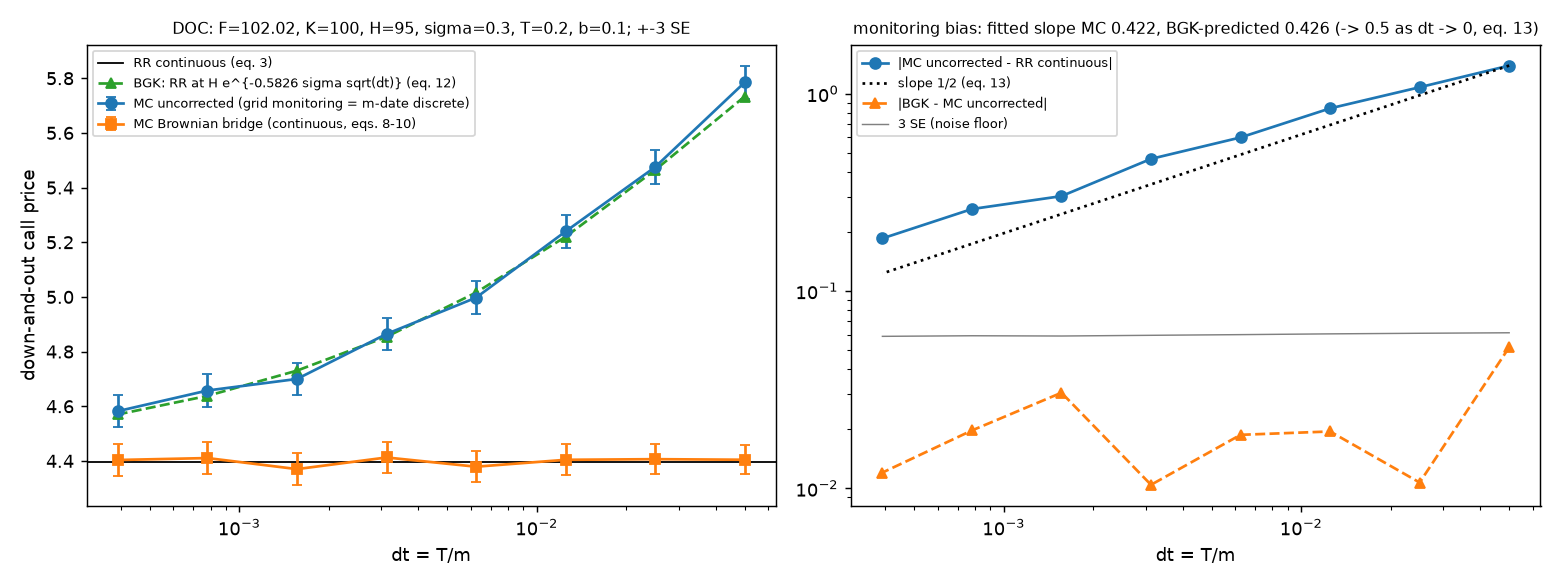
\includegraphics[width=\textwidth]{barrier_mc_vs_rr.png}
\caption{Down-and-out call ($F=102.02$, $K=100$, $H=95$, $\sigma=0.3$, $T=0.2$, $b=0.1$), bars at $\pm3$ SE,
$2\times10^5$ paths per point. Left: naive Monte Carlo (which prices the $m$-date contract), continuous formula at the
BGK-shifted barrier, Brownian-bridge Monte Carlo and continuous formula. Right: naive Monte Carlo bias on a log-log
scale, with estimated slope 0.422 against the line of slope $\frac12$.}
\label{fig:barrier-mc-rr}
\end{figure}

Figure~\ref{fig:barrier-mc-rr} sums it all up. On the left, naive Monte Carlo (blue) slowly falls towards the
continuous price and agrees, within error, with the BGK formula (green): it is pricing the discrete contract. The
Brownian bridge (orange) sits on the continuous formula for every $\Delta t$. On the right, the difference between BGK
and naive Monte Carlo stays below the 3 SE threshold.

\subsection{Where BGK works and where it does not}
Table~\ref{tab:bgk} compares the correction with the published discrete values.

\begin{table}[htb]
\centering
\small
\caption{BGK correction against the discrete price ($K=100$, $\sigma=0.30$, $T=0.2$, $b=0.1$).}
\label{tab:bgk}
\begin{tabular*}{\textwidth}{@{\extracolsep{\fill}}lrrrrrl@{}}
\toprule
case & $m$ & $H$ & true & BGK & relative error & note\\
\midrule
DOC, $S_0=100$ & 50 & 85 & 6.322 & 6.3223 & $+0.11\%$ & \\
DOC & 50 & 95 & 4.907 & 4.9071 & $-0.03\%$ & \\
DOC & 50 & 98 & 3.126 & 3.1210 & $-0.63\%$ & \\
DOC & 50 & 99 & 2.337 & 2.2713 & $-3.10\%$ & close to the barrier\\
DOC & 5 & 99 & 4.489 & 4.0495 & $-9.23\%$ & \\
UOC, $S_0=110$ & 50 & 115 & 0.807 & 0.8188 & $+1.56\%$ & reverse\\
\bottomrule
\end{tabular*}
\end{table}

``True'' is the discrete value published by BGK; the relative error is measured against the project's discrete Monte
Carlo (exact steps at the dates). Far from the barrier the error is a few hundredths of a percentage point. Within
about one step standard deviation of the barrier the correction degrades; there the discrete Monte Carlo is used. By
construction, with the dates on the grid nodes, path by path continuous knock-out $\le$ discrete knock-out.

\section{Barriers under Heston: the bridge on the variance}
Under Heston the same formula \eqref{eq:bb} is used with the variance at the start of the step, $\sigma_i^2=v_i^+$.
\begin{perche}[title={Why the bridge is not exact here}]
Given the variance path, $\ln S$ is Gaussian with a variance that changes over time and a drift that depends on $v$.
Freezing $v$ at its value at the start of the step is the ``local volatility'' rule: it is exact only as
$\Delta\to0$. Moreover, in a step with $v_i^+=0$ the path cannot cross. We therefore expect some exits to be missed
and knock-outs to come out slightly too expensive: a positive bias of order $\Delta$.
\end{perche}
\begin{progetto}[title={In the qpricer project: the measured residual bias}]
Oracle: \eqref{eq:cdo-model-free}, cdo$(K=H=90)=10\,\DF$, on a Heston parameter set that violates Feller (the FO set
of Chapter~\ref{cap:mc}), QE-M scheme. An independent check averaged 25 seeds for each step:
\begin{center}
\small
\begin{tabular}{lcccc}
\toprule
$\Delta$ & 1/32 & 1/64 & 1/128 & 1/256\\
\midrule
bias of cdo $-10\,\DF$ & $+0.095$ & $+0.055$ & $+0.020\pm0.005$ & $+0.012\pm0.005$\\
\bottomrule
\end{tabular}
\end{center}
The bias is of order $\Delta$ and positive, as predicted. The 3 SE test with $2\times10^5$ paths passes at
$\Delta=1/128$ ($z=+0.75$) because $0.020$ is below the standard error of the test (0.024), \emph{not} because the
bias is zero. At $\Delta=1/64$ about 16\% of the seeds would fail. For tighter accuracy $\Delta\le1/256$ is used.
BGK is not used under Heston: discrete contracts are priced with the discrete Monte Carlo.

\smallskip
Second test: with $\xi=10^{-4}$, $\rho=0$ Heston becomes Black with $\sigma=\sqrt\theta$. Maximum $|z|=2.97$ on the
declared seed. It is an unlucky seed (about one in 75): on the same set of paths the vanilla is also off by $-3.15$
and $+3.13$ SE, and the barrier $z$ tracks the vanilla $z$ with correlation 0.905. Over 300 independent seeds the mean
$z$ per cell lies between $-0.031$ and $+0.011$: no bias. The seed was not changed.
\end{progetto}

\section{The case of Haug's table}
Haug's (1998) table is the classic reference for barriers: $S_0=100$, $r=8\%$, $b=4\%$, $T=0.5$, rebate $R=3$,
continuous monitoring. In forward form: $F=100e^{0.02}=102.0201340$, $\DF=e^{-0.04}$, carry $b=0.04$. There are 72
cells (12 type$\times$barrier combinations, three strikes, $\sigma\in\{0.25,0.30\}$) rounded to four decimals, so the
natural tolerance is $5\times10^{-5}$. For example, cdo with $H=95$, $K=100$, $\sigma=0.25$ is worth 6.7924.

\begin{esempio}[title={Example: six published values that do not add up}]
66 cells out of 72 meet $5\times10^{-5}$: maximum $4.96\times10^{-5}$ at $\sigma=0.25$ and $4.59\times10^{-5}$ at
$\sigma=0.30$. Six cells at $\sigma=0.30$, however, are off by $5.2$--$6.25\times10^{-5}$: cuo($H=105$, $K=90$),
puo($H=105$, $K=90,100,110$) and pdi($H=95$, $K=100,110$). For example, puo with $K=90$ is worth $4.22923747$, but the
table prints 4.2293.
\end{esempio}

\paragraph{Suspect the math first.} The rule is to suspect the math first, then the code, and the reference last.
Three mutually independent methods agree on those six cells:
\begin{itemize}
\item direct quadrature of the ``killed'' density and of the first-passage density, without using the algebra of the
building blocks $A$--$\mathcal F$: it agrees with Reiner--Rubinstein to within $3.2\times10^{-14}$;
\item an independent transcription of Reiner--Rubinstein in Haug's spot form;
\item a partial differential equation solved with Crank--Nicolson, which does not use reflection: it agrees with the
spot form to within $5.5\times10^{-10}$.
\end{itemize}
The discrepancies are one unit in the fourth decimal place, and no small perturbation of $(\sigma,T,r,b)$ explains the
column better. Conclusion: those six printed values are not correctly rounded.

\paragraph{How it was handled, without loosening the tolerance.} A first attempt had moved the entire $\sigma=0.30$
column to $10^{-4}$. That was wrong: it also loosened 30 cells that pass at $5\times10^{-5}$. An independent check
flagged it and that version was withdrawn. The final treatment is per cell:
\begin{itemize}
\item the 66 correctly rounded cells stay at $5\times10^{-5}$ against the published value;
\item the six wrong cells are flagged as such in a reference file built with the two independent methods
(\path{tests/golden/barrier_haug.json}) and are tested against that value at $10^{-10}$ (measured
$3.46\times10^{-14}$);
\item all 72 cells are also tested against the reference file at $10^{-10}$ (measured $4.80\times10^{-14}$).
\end{itemize}
The criterion did not change: the reference changed for six cells, and the test became tighter, not looser.

\section{Risks and pitfalls}
\begin{itemize}
\item \textbf{Greeks near the barrier.} A knock-out with a non-zero payoff at the barrier (``reverse'', for example
cuo with $K<H$ or pdo with $K>H$) jumps by $|H-K|$ at the hit. Near expiry delta and gamma explode and the hedge is
not smooth: hedging a discontinuity would require unbounded trades. Vega near the barrier is negative (more volatility
means a higher probability of being knocked out). The price depends on the volatility \emph{at the barrier} and on the
forward skew, not on the ATM volatility: this is why Black and Heston give different prices.
\item \textbf{Finite differences that cross the barrier.} A bump of $S$ that goes past $H$ jumps to the ``barrier
already touched'' branch. The bump must be less than half the distance to $H$; in Monte Carlo common random numbers
are used with the smooth weight $w$, never the discrete indicator.
\item \textbf{Computing $\varrho^{2\mu}\Phi(\cdot)$ with small $\sigma$.} $\mu=b/\sigma^2-\frac12$ is large and the
product can give $\infty\cdot0$. The code works in logarithms:
$\exp\big(2\mu\ln\varrho+\log\Phi(\cdot)\big)$, with \code{log\_ndtr}.
\item \textbf{Negative rates with a rebate.} If $\DF>1$, $\lambda^2=\mu^2+2r/\sigma^2$ can be negative and
$\mathcal F$ does not exist: with $R>0$ an error is raised.
\item \textbf{Many 3 SE tests.} With eight types, several strikes and several barriers, about 0.27\% of the
comparisons fail even with correct code. The seed is fixed, every failure is diagnosed, and the seed is never changed
to make a test pass.
\end{itemize}

\needspace{22\baselineskip}
\begin{progetto}[title={In the qpricer project: code and results}]
The closed-form formula is \code{barrier\_price} in \path{src/qpricer/engines/analytic.py}; the Monte Carlo is
\code{barrier\_mc} in \path{src/qpricer/engines/exotic_mc.py}, with the weight \eqref{eq:peso-bb} computed by
\code{bridge\_survival}. Tests in \path{tests/test_barrier.py}.
\begin{center}
\small
\begin{tabularx}{\textwidth}{>{\raggedright\arraybackslash}Xll}
\toprule
check & measured & threshold\\
\midrule
in + out = vanilla, same paths (8 types, Black and Heston, continuous and discrete) & $3.55\times10^{-15}$ &
$<10^{-12}$\\
Brownian bridge vs Reiner--Rubinstein, 56 cells, $b\in\{0,0.04\}$, $M\in\{1,50\}$ & $\max|z|=1.99$ & 3 SE\\
Heston $\xi=10^{-4}$ vs Reiner--Rubinstein at $\sqrt\theta$ & $\max|z|=2.97$ & 3 SE\\
Heston, cdo$(K=H)=10\,\DF$ at $\Delta=1/128$ & $z=+0.75$ & 3 SE\\
continuous formula and BGK vs BGK tables & $4.97\times10^{-4}$ & $5\times10^{-4}$\\
discrete Monte Carlo vs BGK ``true'' values (13 cells) & $\max|d|/(3\mathrm{SE}+10^{-3})=0.54$ & $\le1$\\
Haug, 66 correctly rounded cells & $4.96\times10^{-5}$ & $5\times10^{-5}$\\
Haug, 6 wrong cells vs independent reference & $3.46\times10^{-14}$ & $10^{-10}$\\
\bottomrule
\end{tabularx}
\end{center}
The cells that must be exactly zero (cuo with $K\ge H$, pdo with $K\le H$) are exactly zero in Monte Carlo as well.
Over 2800 $z$ values obtained with fresh seeds, an independent check found mean $+0.026$, standard deviation 0.998 and
0.36\% beyond 3 (expected 0.27\%).
\end{progetto}

\needspace{6\baselineskip}
\begin{riassunto}
\begin{itemize}
\item Eight types; in + out = vanilla in every model. In Monte Carlo, on the same paths, it holds to rounding.
\item Reflection + Girsanov $\Rightarrow$ reflected world with forward $F^*=\varrho^2F$ and weight $\varrho^{2\mu}$;
the Reiner--Rubinstein formulas are combinations of Black formulas.
\item Zero carry: static hedge with $K/H$ puts of strike $H^2/K$. $\text{cdo}(K=H)=\DF(F-H)$ for every continuous
martingale.
\item Continuous Monte Carlo: weight $\prod(1-p_i)$ with $p_i=e^{-2AC/(\sigma^2\Delta)}$, exact under Black for any
step.
\item Discrete monitoring: barrier shifted by $0.5826\,\sigma\sqrt{\Delta t}$ (BGK). Measured bias slope 0.42: it is
pre-asymptotic, not an error.
\item Under Heston the bridge with $v_i^+$ has a bias of order $\Delta$ (+0.020 at $\Delta=1/128$).
\item Six of Haug's values are wrongly rounded: handled per cell against an independent reference, without loosening.
\end{itemize}
\end{riassunto}

\needspace{9\baselineskip}
\begin{domande}
\begin{enumerate}
\item Why does in + out = vanilla hold in every model? Why must it hold to $10^{-12}$ in Monte Carlo and not within
3 SE?
\item Derive \eqref{eq:immagine} in three steps (Girsanov, reflection, symmetry).
\item Derive the crossing probability \eqref{eq:bb} and show that the drift cancels.
\item Why does the weight $w$ have lower variance than the drawn uniform?
\item Why is a knock-out with a daily-observed barrier worth more than one with a continuous barrier? Where does
$0.5826$ come from?
\item The measured slope is 0.42 instead of 0.5: what do you check before calling it an error?
\item What is special about the down-and-out call with $K=H$ at zero carry? Why is it useful under Heston?
\item Six published values fail the tolerance. How do you proceed?
\end{enumerate}
\end{domande}
